\documentclass[compsoc,onecolumn]{IEEEtran}
% *** GRAPHICS RELATED PACKAGES ***
%

\ifCLASSINFOpdf
  \usepackage[pdftex]{graphicx}
  % declare the path(s) where your graphic files are
  \graphicspath{{fig/}}
  % and their extensions so you won't have to specify these with
  % every instance of \includegraphics
  % \DeclareGraphicsExtensions{.pdf,.jpeg,.png, .bmp}
\else
  % or other class option (dvipsone, dvipdf, if not using dvips). graphicx
  % will default to the driver specified in the system graphics.cfg if no
  % driver is specified.

   \usepackage[dvips]{graphicx}
  % declare the path(s) where your graphic files are
   \graphicspath{{eps/}}
  % and their extensions so you won't have to specify these with
  % every instance of \includegraphics
   \DeclareGraphicsExtensions{.eps}
\fi
\usepackage{natbib}
\usepackage[bookmarks=false]{hyperref}
\usepackage{mathtools}
\usepackage{amssymb,amsmath}
\usepackage{textcomp}
\usepackage{url}
\usepackage{caption}
\usepackage{subcaption}
\usepackage{tabulary}
\usepackage{setspace}

\usepackage{balance}
\usepackage{flafter}
%\usepackage[linesnumbered,ruled]{algorithm2e}
%\usepackage{algorithmic}
%\usepackage{algorithm}
\usepackage[linesnumbered,ruled]{algorithm2e}
\usepackage{algpseudocode}
\usepackage{amsmath}
\usepackage{varwidth}
\SetKwInOut{Input}{Input}
\SetKwInOut{Output}{Output}
\usepackage{color}
\newcommand\todo[1]{\textcolor{blue}{(todo : #1)}}
\DontPrintSemicolon

%\usepackage{algorithm2e}
%\usepackage{amsmath}
%\usepackage[linesnumbered,ruled]{algorithm2e}
%\usepackage[ruled,vlined,linesnumbered]{algorithm2e}



% This allows align equations to be broken across pages
\allowdisplaybreaks
% correct bad hyphenation here
\hyphenation{op-tical net-works semi-conduc-tor}

\doublespacing
\begin{document}

\title{Using Knowledge Distillation As A Possible Solution For The Domain Transfer Problem In Fact Verification }

% author names and affiliations
% use a multiple column layout for up to two different
% affiliations

\author{\IEEEauthorblockN{}
\IEEEauthorblockA{Mithun Paul\\
}
}


% use for special paper notices
%\IEEEspecialpapernotice{(Invited Paper)}

% make the title area
\maketitle



\section{Problem Statement}
Neural networks (NNs)  play a key role in in most natural language processing systems with state of the art (SOA) performance \citep*{devlin2018bert, sun2018improving,bohnet2018morphosyntactic} especially in the domain of recognizing textual entailment \citep*{kim2018semantic}, fake news detection \citep*{baird2017talos} and fact verification \citep*{nie2018combining}.
The task of natural language inference is considered to be an integral part of natural language understanding (NLU). In this task, which can be seen as a particular instance of recognizing textual entailment (recognizing textual entailment) \citep*{fyodorov2000natural,condoravdi2003entailment,bos2005recognising,maccartney2009extended}, a model is asked to classify if a given sentence (premise) \textit{entails}, \textit{contradicts} or is \textit{neutral} given a second sentence (hypothesis).

Here I focus on the recognizing textual entailment (recognizing textual entailment) task \citep*{dagan2013recognizing}, and its application to fact verification \citep*{thorne2018fever}.

In the world of natural language understanding, recognizing textual entailment (recognizing textual entailment) is the task of determining if one piece of text can be plausibly inferred from another. In the Fact Extraction and Verification (FEVER) shared task \citep*{thorne2018fever}, the recognizing textual entailment module was used determine if a given set of evidence sentences, when compared with the claim provided, can be classified as \textit{supports, refutes}, or \textit{not enough information}.


However, I suspect that these models depend heavily on lexical information that may transfer poorly between different domains. For example, in early experiments in the fact verification space, I observed that out of all the statements containing the phrase ``American Author,'' 91\% of them belonged to one class label. Such information could be meaningful in the literature news domain, but transfers poorly to other domains such as science or entertainment. 



\subsection{Related Work}

it has been shown that these models also learn from the subtle biases inherent in these datasets \citep*{gururangan2018annotation}.



In order to advance any natural language processing task, quality data sets are quintessential. Some such data sets which have enabled the advancement of natural language inference (and fact verification) are SNLI \citep*{bowman2015large} MNLI \citep*{williams2017broad}, FEVER \citep*{thorne2018fever}, and FNC \citep*{pomerleau2017fake}.

However these datasets are not devoid of biases (subtle statistical patterns in a dataset, which could have been introduced either due to the methodology of data collection or due to an inherent social bias). 
For example, \citep*{gururangan2018annotation} and \citep*{poliak2018hypothesis} show that biases were introduced into the MNLI dataset by certain language creation choices made by the crowd workers. Similarly, \citep*{schuster2019towards} show that in the FEVER, the REFUTES label (same as the \textit{contradicts} label mentioned above) highly correlates with the presence of negation phrases. 

These biases can be readily exploited by neural networks (NNs), and thus have influence on performance.  As an example, \citep*{gururangan2018annotation} demonstrate that many state of the art methods in natural language inference could still achieve reasonable accuracies when trained with the hypothesis alone. Similarly, \citep*{emnlp2019sandeep} show that some neural network methods with very high performance accuracies are heavily dependent on lexical information. This tendency of NNs to inadvertantly exploit such dataset artifacts is likely worsened by the fact that currently the success of natural language processing approaches is almost exclusively measured by empirical performance on benchmark datasets. While this emphasis on performance has facilitated the development of practical solutions, they may lack guidance as they are often not motivated by more general linguistic principles or human intuition. This makes it difficult to accurately judge the degree to which these methods actually extract reasonable representations, correlate with  human intuition or understand the underlying semantics~\citep*{dagan2013recognizing}.


 
In this work I postulate that altering these datasets based on lexical importance is beneficial for organizing research and guiding future empirical work. While the technique of delexicalization (or masking) has been used before~\citep*{zeman2008cross}, I have expanded it by incorporating semantic information (the assumption that meaning arises from a set of independent and discrete semantic units)~\citep*{peyrard2019simple}. Since these techniques are general and compatible with most existing semantic representations, I believe they can be further extended onto datasets used for other natural language processing tasks. Thus, by enabling integration of these techniques into the training pipeline, I hope to control lexicalization in the datasets which the neural network methods possibly depend upon. 



 
In this work I postulate that altering these datasets based on lexical importance is beneficial for organizing research and guiding future empirical work. While the technique of delexicalization (or masking) has been used before~\citep*{zeman2008cross}, I have expanded it by incorporating semantic information (the assumption that meaning arises from a set of independent and discrete semantic units)~\citep*{peyrard2019simple}. Since these techniques are general and compatible with most existing semantic representations, I believe they can be further extended onto datasets used for other natural language processing tasks. Thus, by enabling integration of these techniques into the training pipeline, I hope to control lexicalization in the datasets which the neural network methods possibly depend upon. 


\section{Preliminary Work}


In this section I describe several preliminary experiments I conduct to verify that models trained on lexicalized data transfer poorly across domains. In particular I investigate the attention weights a state of the art recognizing textual entailment method~\citep*{parikh2016decomposable} assigns to input tokens in the recognizing textual entailment component of fact verification systems, and confirm that most of the weight is assigned to POS tags of nouns (e.g., neural network, NNP etc.) or their phrases, which verify my ``American Author" observation stated above. Further I also show results from a few proposed solutions which control for unnecessary lexicalization enabling data transfer across domains.



\subsection{Experiment Set-Up}
 
To verify that models trained on lexicalized data transfer poorly, I implement a domain transfer experiment where a state-of-the-art recognizing textual entailment model is trained on one dataset (FEVER \citep*{thorne2018fever}) and tested on another dataset (Fake News Challenge \citep*{pomerleau2017fake}). In particular, the neural network method I use is the Decomposable Attention (DA) \citep*{parikh2016decomposable}, which consistently achieves near state-of-the-art performance on recognizing textual entailment tasks \footnote{This experiment was initially setup during the 2018 FEVER shared task which had provided Decomposable Attention as a strong baseline. At the completion of the shared task, most of the winning teams used another model \citep*{chen2016enhanced}. However, the aim of my work is not to outperform the state of the art performance, but rather to generalize to new domains without retraining.}.  I use the AllenNLP \footnote{\url{https://github.com/allenai/allennlp}}
implementation of DA, which was provided by the FEVER task organizers. To investigate DA's reliance on lexical information, I first examine its word-level attention weights (Section \ref{attention_analysis}). 
Informed by these results, I propose several methods to mask the lexicalized data (Section \ref{masking_techniques}), and evaluate them in in-domain and  out-of-domain settings (Section \ref{sec:results}).




\begin{table}
    \centering
    \footnotesize
    \begin{tabular}{ccccc}
        Dataset & Support & Refute & Discuss & Unrelated \\
        \hline
        FNC    & 5,581 & 1,537  & 13,373 & 54,894 \\
        FEVER  &  86,701 & 36,441  & \multicolumn{2}{c}{42,305 (\textit{NEI})} \\  
    \end{tabular}
    \caption{Label distribution for the FEVER and FNC datasets.  I consider the \textit{agree} and \textit{disagree} FNC labels as equivalent to the \textit{support} and \textit{refute} labels in FEVER. The FNC \textit{not enough info (NEI)} label is listed below the more fine-grained \textit{discuss} and \textit{unrelated} FEVER labels.  }
    \label{tab:data}
\end{table}

\subsection{Datasets}
I use two distinct fact verification datasets for my experiments :

{\flushleft{\bf Fake News Challenge (FNC):}} 
The FNC dataset~\citep*{pomerleau2017fake} contains four classes (\textit{agree}, \textit{disagree}, \textit{discuss}, and \textit{unrelated}) and has publicly available training (49,972 data points) and test partitions (25,413 data points). Each data point consists of a claim and a set of evidence sentences.  I split the training dataset into two partitions, with 40,904 records for training and 9,068 records for development.

{\flushleft{\bf Fact Extraction and Verification (FEVER):}} The FEVER \citep*{thorne2018fever} dataset consists of 145,449 training data points, each of which has a claim and a set of evidences retrieved from Wikipedia using a baseline information retrieval (IR) module.
The FEVER claim-evidence pairs were assigned labels from three classes: \textit{supports}, \textit{refutes}, and \textit{not enough info (NEI)} . Even though the partition of the FEVER dataset that was used in the final shared task competition was released publicly, the gold test labels were not. Hence I used the development portion (19,998 data points) instead as my test partition. I created my own development partition by randomly dividing the training partition into 80\% for training (119,197 data points) and 20\% (26,252 data points) for development.  The evidence for data points that had the gold label of \textit{not enough info} can be retrieved (using a task-provided IR component) either by finding the nearest neighbor to the claim or randomly \citep*{thorne2018fever}. 


\subsubsection{Cross-domain Labels}
\label{sec:crossdomain}


In order to evaluate models in a cross-domain setting, I modified the label space of the source domain to match that of the target domain. This  also allows us to evaluate using the official scoring measures of the target domain. In particular, when training on FEVER and testing on FNC, the data points in FEVER that belong to the class \textit{supports} were relabeled as \textit{agree}, and those in \textit{refutes} as \textit{disagree}. The data points belonging to the third class \textit{NEI} were divided into \textit{discuss} and \textit{unrelated} as follows.
In the FEVER dataset, two separate methods were used to retrieve the evidence sentences for the class \textit{NEI}: 1) sampling a sentence from the nearest page to the claim as evidence using their document retrieval component, and 2) sampling a sentence from Wikipedia uniformly at random. The evidence sentences retrieved using the nearest page technique were assigned the label \textit{discuss} (since it was more likely to be topically relevant to the claim), and the rest were assigned the label \textit{unrelated}. Also the distribution of labels was made similar to that of FNC. In particular, 16.86\% of the total 35,639 data points that originally belonged to the class NEI in FEVER were thus assigned the label \textit{discuss} and the rest (83.14\%) were assigned the label \textit{unrelated}. For the experiments in the opposite direction, i.e., when training on FNC and testing on FEVER, I collapsed the \textit{unrelated} and \textit{discuss} classes into a single class, \textit{not enough info} (see Table~\ref{tab:data} for a summary on label distribution).


\subsection{Error Analysis of Cross-Domain Attention}\label{attention_analysis}


I use the word-level attention weights~\citep*{bahdanau2014neural} learned by DA to perform  an error analysis in the cross-domain evaluation. 
In particular, I first trained two equivalent DA models, one on FEVER and the other on FNC. 
Next, I used both models to predict instances in FEVER development. For each data instance, I calculated the cumulative attention weights assigned by each of the two models to all evidence words. 
For each of the data instances that were {\em incorrectly} classified by the model trained out of domain (i.e., on FNC) and were {\em correctly} classified by the in-domain model, 
I  selected the words that were present in the set of top three words with the highest attention score according to the out-of-domain model, but were {\em not} present in the equivalent set produced by the in-domain model. Such words indicate potential overfitting of the out-of-domain model. 
Figure \ref{fig:attention} shows the distribution of part-of-speech (POS) tags for these words. The figure indicates that, for incorrectly classified examples in cross-domain, the higher attention weights were assigned to nouns.
Importantly, 43.10\% of these noun phrases in FEVER are named entities. 



\begin{figure}
 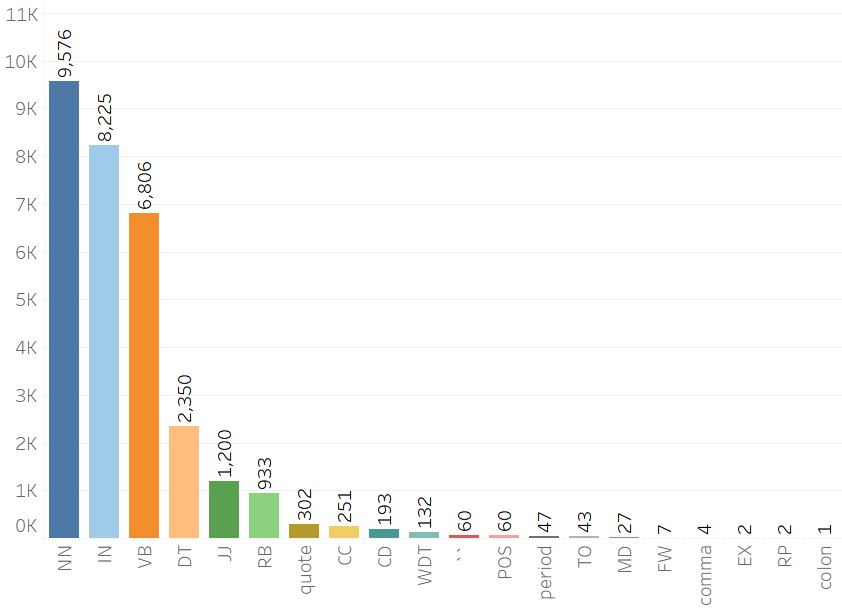
\includegraphics[width=0.95\linewidth]{histogram_2.jpg}
    \vspace{-3mm}
    \caption{ Distribution of POS tags that were assigned the highest attention weights by DA for incorrectly classified cross-domain examples.}
  \label{fig:attention}
\vspace{-6mm}
\end{figure}



 With this analysis, I was able to confirm that most of the weight is assigned to POS tags of nouns or elements of noun phrases, which confirms my observation that these models anchor themselves on lexical information that is more likely to be domain dependent. 
 As expected, even though this method achieves high accuracy when evaluated in the same domain, the performance in the target domain is poor, marginally above chance.






\subsection{Proposed Solutions}
To mitigate the potential domain dependence introduced by these large attention weights, I propose several semantic masking techniques, which I compare with a deletion baseline.  
Particularly I experiment with several strategies for delexicalization, i.e., where lexical tokens are replaced (or masked) with indicators of their class. While the technique of delexicalization/masking has been used before \citep*[e.g.,]{zeman2008cross}, here I expand it by incorporating semantic information. In particular, I first replace named entities with their corresponding semantic tags from Stanford's CoreNLP \citep*{manning2014stanford}. 
To keep track of which entities are referenced betIen claim and evidence sentences, I extend these tags with unique identifiers. Second, I similarly replace other word classes in the sentence (common nouns, verbs, adjectives, and adverbs)  with their super sense tags \citep*{ciaramita2003supersense}.

\subsubsection{Masking Techniques} \label{masking_techniques}
In this section I describe in detail various masking techniques which were used in the experiments. Examples of each form of masking are shown in Table~\ref{masking_examples}.


\begin{table*}[t]
\begin{center}
\begin{tabular}{p{20mm}|p{55mm}|p{70mm}}

\textbf{Config.} & \textbf{Claim}& \textbf{Evidence} \\ \hline
Lexicalized & {With Singapore Airlines, the Airbus A380 entered commercial service.} & {The A380 made its first flight on 27 April 2005 and entered commercial service on 25 October 2007 with Singapore Airlines.}\\
\hline 
NE Deletion & {With  , the  entered commercial service.} & {The A380 made its  flight on  and entered commercial service on  with.}\\
\hline 
Basic NER  & {With \texttt{organization}, the \texttt{miscellaneous} entered commercial service.} & {The A380 made its \texttt{ordinal} flight on \texttt{date} and entered commercial service on \texttt{date} with \texttt{organization}.}\\
\hline 
OA-NER  & {With \texttt{organization-c1}, the \texttt{misc-c1} entered commercial service.} & {The A380 made its \texttt{ordinal-e1} flight on \texttt{ date-e1} and entered commercial service on \texttt{date-e2} with \texttt{organization-c1}.}\\
\hline 

\mbox{OA-NER+SS} Tags & {With \texttt{organization-c1}, the \texttt{artifact-c1} \texttt{motion-c1} commercial \texttt{act-c1} .} & {The A380 \texttt{stative} its \texttt{ordinal-e1 cognition-e1} on \texttt{date-e1} and \texttt{motion-c1} commercial \texttt{act-c1 on date-e4} with \texttt{organization-c1}.  
}\\

\end{tabular}
\end{center}

    \caption{ Example illustratingmy various masking techniques, compared to the original fully lexicalized data. Note that the masking tags were generated with real-world (imperfect) tools. For example, "Airbus A380" in the claim was correctly classified as \texttt{miscellaneous} by the NER tool, while ``A380" in the evidence was not, thus preventing us from taking advantage of the overlap. }
    \label{masking_examples}
\end{table*}

{\flushleft{\textbf{Named Entity (NE) Deletion Baseline:} }}
Lexical items which are tagged as named or numeric entities (NE) by CoreNLP's named entity recognizer (NER)~\citep*{manning2014stanford} are deleted.  

{\flushleft{\textbf{Basic NER:}}}  Token sequences which are labeled as NEs are replaced by the corresponding label, e.g., \texttt{location, person}.

{\flushleft{\textbf{Overlap Aware NER (OA-NER)}: }} This technique additionally captures the \textit{lexical overlap} between the claim and evidence sentences with entity ids.  
That is, the first instance of a given entity in the claim is tagged with \texttt{c1}, where the \texttt{c} denotes the fact that it was found in the claim sentence (e.g., \texttt{person-c1}). Wherever this {\em same} entity is found later, in claim or in evidence, it is replaced with this unique tag. If an entity is found only in evidence, then it is denoted by an \texttt{e} tag. (e.g., \texttt{location-e3} would be the third location found only in the evidence).

For example, in the claim-evidence pair shown in Table~\ref{masking_examples}, when the named entity \textit{Singapore Airlines} appears in the claim it is replaced with \texttt{organization-c1}, since it is the first \texttt{organization} to appear in claim. 
The same id is used wherever the same entity is seen again, e.g., in the evidence sentence. However, the date \textit{27 April 2005} occurs only in the evidence, and hence it is replaced with \texttt{date-e1}.
Importantly, I create pseudo-pretrained embeddings for these new OA-NER-based tokens by adding a small amount of random Gaussian noise (mean 0 and variance of 0.1) to pre-trained embeddings~\citep*{pennington2014glove} of the root word corresponding to the category (e.g., \textit{person}). Thus the embeddings of all the sub-tags, while being unique, are close to that of the root word.
{\flushleft{\textbf{OA-NER + Super Sense (SS) Tags}}}:
Super-sense tagging is a sequence modeling approach that annotates phrases with coarse WordNet senses~\citep*{ciaramita2003supersense}~\citep*{miller1990introduction}. In this masking method, I not only replace named entities with their OA-NER tags, but also replace other lexical items with their corresponding super sense tags, if found. As with the OA-NER approach, the lexical overlap is also explicitly marked for all these tags with unique ids (see Table~\ref{masking_examples}). 


\begin{table*}[ht]
\begin{center}
\begin{tabular}{p{22mm}|p{9mm}p{9mm}p{9mm}p{9mm}}
 & \multicolumn{4}{c}{Configuration} \\
 \hline
Train Domain & {FNC}& {FEVER}  & {FEVER} & {{FNC}} \\ 
Eval Domain & {FNC}& {{FNC}}  & {FEVER} & {{FEVER}} \\ \hline
Masking & & & & \\
\hline
Lexicalized &68.99\%& {48.86\%} &83.43\%& {41.16\%} \\
%\hline
Deletion  &66.45\%& 40.23\% &75.34\%& 33.33\% \\
%\hline
Basic NER &69.40\%& 46.27\% &76.23\%& 35.72\%\\
%\hline 
\textbf{OA-NER} &65.85\%& \textbf{53.59}\% &{82.31\%}& {46.47\%}\\
%\hline 
\textbf{OA-NER+SS} & 45.51\%& 46.71\% &75.26\%& {\bf 51.77\%}\\
\end{tabular}
\end{center}
    \caption{\label{crossdomain} Various masking techniques and their performance accuracies, both in-domain and out-of-domain.} \label{tab:results}

\end{table*}


\subsection{Results} 
\label{sec:results}
The evaluation of the proposed masking strategy on the two fact verification datasets indicates that,
while the in-domain performance remains on par with that of the model trained on the original, lexicalized data, it improves considerably when tested in the out-of-domain dataset. 
For example, the performance of a state-of-the-art recognizing textual entailment model trained on the masked FNC data and evaluated on FEVER data improved by over 10\% in accuracy score compared to the fully lexicalized model. Similarly, the model trained on the masked FEVER data and tested on FNC outperforms the lexicalized model by 4.7\% FNC score.
Thus my experiments demonstrate that my masking strategy is successful in mitigating the dependency on domain-specific lexical information.

recognizing textual entailment is the task of determining if one piece of text can be plausibly inferred from another. In the Fact Extraction and Verification (FEVER) shared task \citep*{thorne2018fever}, the recognizing textual entailment module was used determine if a given set of evidence sentences, when compared with the claim provided, can be classified as \textit{supports, refutes}, or \textit{not enough information}.


Table~\ref{results} shows the performance of each of these methods (DA and ESIM) on  both the lexicalized and delexicalized versions of the MNLI dataset. As shown in the table, the accuracies of both the methods increase when trained with the delexicalized version of the dataset. This aligns with my intution that delexicalization helps towards de-biasing these datasets, and thus preventing the neural network methods from being \textit{distracted} by  statistical patterns that are not meaningful for the task at hand.
 
While the ability of a neural network method to derive reasonable representations within the training domain is important, it is also important to have the ability to transfer across domains. Hence, to test the effect of delexicalization on domain transferability I picked one of the methods, decomposable attention (DA), trained it in one domain and tested it in an out-of-domain setting (the DA was chosen since it was provided off-the-shelf with FEVER baseline code). These results can be seen in Table ~\ref{results_outofdomain}. Specifically, the table shows the accuracies in three settings, i.e., when the model was trained on MNLI and then tested on MedNLI datasets, when it was trained on FNC and  tested on the FEVER datasets, and when the model was trained on FEVER and tested on FNC datasets. Note that in some cases of out-of-domain experiments, the label space of the source domain did not match with that of the target domain. Specifically, while the FEVER dataset consisted of data belonging to 3 classes, the FNC dataset had data points belonging to 4 classes. To enable us to evaluate using the official scoring measures of a target domain, I followed the label alignment approach used in \citep*{emnlp2019sandeep}. For example, while the data points that belonged to the class \textit{supports} were mapped to \textit{agree}, and \textit{refutes} to \textit{disagree}, the ones in the class \textit{not enough info} were further divided to align with the \textit{unrelated} and \textit{discuss} labels.

The experiments summarized in these tables highlight three observations: (a) The models trained on delexicalized data do not perform worse than the ones trained using lexicalized datasets; (b) in the two settings with texts where the named entities discussed are well covered by the NER used in this work (from FEVER to FNC, and from FNC to FEVER), the results demonstrate that the semantic lifting provided by my OA-NER method improves domain transfer considerably; and (c) I do not see a significant improvement in the transition from MNLI to MedNLI.  I suspect this is because of the limited overlap of named entity types between the MedNLI and MNLI. For example while the named entity recognizer (CoreNLP) I used, focuses on PERSON, ORGANIZATION, etc. the MedNLI dataset contains more medical terms related diseases and symptoms. This possibly necessitates the importance of exploring using a domain-relevant NER.



\begin{table*}[h]
\begin{center}
\begin{tabular}{|p{20mm}|p{20mm}|p{20mm}|p{20mm}|p{20mm}|p{20mm}|p{20mm}|}
\hline 
\textbf{Method} & \textbf{MNLI matched lexicalized }& \textbf{MNLI matched delexicalized } & \textbf{MNLI mismatched lexicalized } &\textbf{MNLI mismatched delexicalized } \\
 \hline
DA & {60.95\%} &{64.52\%} &{61.43\%}&{64.86\%}\\
\hline 
ESIM  & {68.84\%} &{68.14\%} &{69.40\%}&{69.10\%}\\
\hline 
\end{tabular}
\end{center}
\caption{Performance of various high performing neural network methods over lexicalized and delexicalized versions of the same dataset. `Matched' is the in-domain partition of the MNLI validation dataset, and `mis-matched' is the out-of-domain partition. The performance of both the methods remain close to each other in delexicalized and lexicalized versions of the same dataset, which validates that my  delexicalization techniques preserve the original information of the text. }

    \label{results}
\end{table*}



\begin{table*}[h]
\begin{center}
\begin{tabular}{|p{25mm}|p{12mm}|p{11mm}|p{10mm}|}
 \hline
\textbf{Train Domain} & \textbf{MNLI}& \textbf{FEVER}   & \textbf{FNC} \\ 
 \textbf{Eval Domain} & \textbf{MedNLI}& \textbf{{FNC}}   & \textbf{{FEVER}} \\ 
\hline
Lexicalized &51.47\%& {48.86\%} & {41.16\%} \\
OA-NER &51.57\%& 53.59\% & {46.47\%}\\
\hline
\end{tabular}
\end{center}
    \caption{ Performance accuracies of the Decomposable Attention against various masking techniques when tested out-of-domain. The ``Train Domain'' row indicates the training datasets, while the ``Eval Domain'' indicates the domain of the corresponding evaluation partitions. For example, one experiment trained the DA method on FEVER and evaluated the resulting model on the testing partition of FNC (column 3). }
    
    \label{results_outofdomain}
\end{table*}


\begin{table*}[h!]
\begin{center}
\begin{tabular}{|p{20mm}|p{9mm}|p{10mm}|}
 \hline
\textbf{Masking strategy} & \textbf{FNC}  & \textbf{FEVER}  \\ 
\hline
Lexicalized &68.99\% &83.43\% \\
OA-NER &65.85\% &82.31\%\\
OA-NER+SS & 45.51\% &75.26\%\\
\hline
\end{tabular}
\end{center}
    \caption{Performance accuracies of the Decomposable Attention against various masking techniques when tested in-domain for FNC and FEVER datasets. The ``Lexicalized" row shows the accuracies when DA was trained using the corresponding lexicalized data. This demonstrates that while delexicalization with OA-NER maintains the performance, the addition of Super Sense tags reduces the accuracy, emphasizing the fact that the amount of granularity to use is still an open problem.}
    \label{sstag}
\end{table*}


\section{Future Work/Plan for Dissertation}
In the previous sections I investigate the need for delexicalization techniques to reduce the potential dependence of neural network methods on lexicalized items in natural language inference tasks. My experiments show that delexicalization achieves comparative results {\em in-domain} with the state of the art methods trained on lexicalized data. Importantly, I show that methods trained on delexicalized data transfer considerably better {\em out-of-domain}, which  confirms the importance of delexicalization in natural language inference tasks for domain transferability.

In this section I describe a few proposed solutions where I explore combining delexicalization with knowledge distillation to transfer learning across domains.





\subsection{Knowledge Distillation of Data}
Knowledge distillation is a training procedure where one neural network method functions as a \textit{teacher} and transfers its knowledge to a \textit{student} model. While the suggestion for knowledge distillation was introduced in \citep*{ba2014deep} it was formally introduced in \citep*{hinton2015distilling}. The motivation behind knowledge distillation is to 


\
\subsection{Discussion of learning temperatures}

\subsection{Proposed Solution}

In this work, I propose to distill the student model from one or more teachers. Specifically, the teacher model will learn from the lexicalized version of a given dataset, while the student model will from the corresponding delexicalized version. 
The reasons for this setup are :

\begin{itemize}
  \item The distilled model learns a more universal language representation by leveraging the cross-lexicalized-delexicalized data.
  \item The student model will achieve comparable accuracy in an in-domain setting.
  \item Since the proposed framework is quite general, where the data of the student model is independent of the teacher model, this possibly can enable the transfer of knowledge across domains.
\end{itemize}

Motivated by the above reasons, I plan to apply knowledge distillation towards solving the domain- transfer problem mentioned above. This is inspired from the idea that datasets in similar domains are possibly related by means of a common low dimensional semantic representation. I propose that using the shared structure within a student teacher model could possibly help by assuming some connections over the underlying data distribution of different datasets. Although many of the recent KD works \citep*{jiao2019tinybert,tang2019distilling,zhao2019extreme}  employ a  pretrained language model as the underlying neural network architecture, I plan to choose simple attention based models adapted from ~\citep*{parikh2016decomposable} and \citep*{chen2016enhanced} . The reasons are:

\begin{itemize}
  \item Both these models have been proven to achieve state of the art results in natural language inference related tasks especially due to their inherent attention mechanisms.
  \item Our approach is more data driven and hence simpler transparent models will enable me to focus on the important semantic transitions (e.g.,choice of different masking methods, influence of KD in domain transfer, etc.) required for data distillation.
 \end{itemize}

\subsection{Related Work}

\todo: find top 5 citations of hinton paper

Many previous methods using knowledge distillation (KD) focus on task-specific KD, which transfers knowledge from a single-task teacher to its student. More recently in Sun et al. \citep*{seo2016bidirectional} , Jiao et al. \citep*{jiao2019tinybert}, and Zhao et al.\citep*{zhao2019extreme}, Tang et al. \citep*{tang2019distilling} the KD algorithms are specially designed
for transformer-based architectures, and the student models are adapted from teacher models. On the other hand Liu et al. \citep*{liu2019attentive}, explore the knowledge distillation method under the setting of multi-task learning \citep*{caruana1997multitask} \citep*{baxter2000model}.

To the best of my knowledge no similar work on using student teacher architecture for data distillation has been done before.
\subsubsection{Proposed Experiment Set-Up}

\subsubsection{Experiment Variations}

\subsubsection{EMA}
\subsubsection{Semi Supervised}
\subsubsection{Weight Tuning}





\subsection{Mean teacher}

\subsection{domain adaptation }




In the next few months I am aiming to do more tests on state of the art models (ESIM, BERT etc) and other standard datasets (MNLI, MEDNLI etc)  to confirm that the problem/proposed hypothesis exists. Also, in my meeting with Dr. Barnard he had suggested that I should further explore the distribution of data labels to confirm the hypothesis. Dr. Morrison similarly had suggested that I should explore the meta learning frameworks like MAML and REPTILE as possible solutions. Between Jan 2020 and March 2020, I will be incorporating these suggestions along with working on a potential solution based on mean teacher framework. A detailed plan, where specific tasks are mapped to conference deadlines, is as below:

\subsection{Amount of generalization}
Also this work touches upon questions about which granularity offers a good approximation of semantic meanings. For example, Table ~\ref{sstag} shows the performance of Decomposable Attention against various delexicalization strategies. It can be seen that, while the addition of OA-NER tags does not change the performance significantly, the semantic lifting provided by the SS tags decreased the accuracies considerably in both cases (FEVER and FNC).  This demonstrates that while generalizing away from lexical items is important, {\em how much} to generalize remains an open research problem.

One future direction of interest is exploring the right level of masking granularity needed for delexicalization, which is likely dependent on the task. 

\section{Conclusion}
 To mitigate this dependence on lexicalized information, I experiment with several strategies for masking out names by replacing them with their semantic category, coupled with a unique identifier to mark that the same or new entities are referenced between claim and evidence. The results show that, while the performance on the FEVER dataset remains at par with that of the model trained on lexicalized data, it improves significantly when tested in the FNC dataset. Thus my experiments demonstrate that my strategy is successful in mitigating the dependency on lexical information.

my experiments show that delexicalization achieves comparative results {\em in-domain} with the state of the art methods trained on lexicalized data. Importantly, I show that methods trained on delexicalized data transfer considerably better {\em out-of-domain}, which  confirms the importance of delexicalization in natural language inference tasks for domain transferability. While there is still room for exploration in delexicalization techniques, I present this methodology as a means  to conduct more meaningful machine learning experiments. To facilitate this, I release the delexicalized versions of MNLI, FEVER and FNC datasets.





\balance
\begin{spacing}{0.88}
%\bibliographystyle{IEEEtran}
\bibliographystyle{unsrtnat}
\bibliography{compre_masking}
\end{spacing}

% that's all folks
\end{document}